\documentclass[11pt,a4paper]{article}
\usepackage{ls}
\usepackage[english]{babel}
\setlist{noitemsep}

\title{Supply Chains and SCOR -- the Supply Chain\\ Operations Reference
  Model} 

\author{Hans-Gert Gr\"abe}

\date{November 21, 2021}

\begin{document}
\maketitle

\section{On the Systemic Structure of (Enterprise) Organisations}

The systemic understanding of an (entreprise) organisation, which can be read
off from the normative documents (APQC-PCF) and practically relevant
enterprise modelling (Business TRIZ) examined so far, assumes two systemic
levels to be distinguished -- operational and strategic management.

From the \emph{perspective of strategic management}, the system is the whole
enterprise, divided into strategic business units as components (APQC-PCF
levels \emph{category} and \emph{process group}). Reduction to essentials at
this level means organising the relationships both between these components
and with the company's environment to achieve the \emph{strategic
  goals}\footnote{According to previous discussions, I use the term
  \emph{goal} for longer-term and \emph{objective} for shorter-term targets.}.
It is therefore a matter of organising the throughput of energy, material (in
the broadest sense, including \enquote{human resources} which play a central
role here) and information in the qualities, quantities and rhythms required
within a specific intrinsically defined time horizon (the \enquote{rhythm} of
the overall system). This kind of organisation assumes that short-wave
temporal fluctuations of the throughput can be intercepted and compensated
within the components. Such \emph{resilience} of the components is, of course,
a property that in turn must be reproduced at the level of the overall
system. APQC-PFC provides here for a company-wide division into 13
\emph{categories} as strategic business areas. These do not have to be
formally established or separated within the company, but if a company wants
to participate in the cross-company exchange of experience that APQC
organises, then these areas must be at least virtually delimitable in the
business model of the company.

The focus of \emph{operational management} is on the concrete design and
development of these individual business areas at the operational and thus at
an intrinsically shorter time horizon.  APQC postulates at that level clearly
more centralised management structures with corresponding authorisations and
rights of intervention, but also responsibilities. On the other hand, it also
provides for differently designed intra-company structures through
\emph{variants of the standard} at the level of modelling processes,
activities and tasks. The standardisation efforts are thus directed at the
\emph{strategic structural level} and a certain standardisation of
\emph{operational processes in their methodological meta-model} rather than
structural model dimension. The latter makes it possible, despite structurally
different modelling at the operational level, to organise the comparison
between process planning and real-world process execution as a contradiction
between \emph{justified expectations} and \emph{experienced results} in a
comparable way by regularly recording \emph{Key Perfomance Indices} (KPI) (see
13.6 \emph{Measure and Benchmark} in APQC-PCF).

This information, collected \emph{globally} at the subsystem level as a
component of the overall system, is then used for controlling processes at the
subsystem level by operational management. This information is thus part of a
\emph{global conceptualisation} for this subsystem level, of a
\emph{cooperative world view} as an emergent phenomenon, which is inseparably
linked to the development and strenghtening of the structure at this subsystem
level.  Both individual steering impulses for individual employees (management
by objective, management by incentive, ...) and cooperative steering tools
(such as the relationships between \emph{Product Owner}, \emph{Team} and
\emph{Scrum Master} in Scrum) are used.

Even if the KPIs are modelled and collected globally throughout the company,
the possible uses of these instruments remain the same at the operational
level, because the authorisation of the operational management is limited
accordingly and thus \emph{judgement practices} can be executed only within
the subsystem. On the other hand, the KPIs of a globally collected system are
not very useful in this level of detail at the strategic management level and
must be \emph{aggregated into strategic KPIs} to enable similar judgement
practices at the strategic level. Such judgement practices at the strategic
level thus strenghten a \emph{strategic worldview} of the company that differs
from the worldview at the operational level in the sense of the tension
between the general and the special. It should be further noted that
operational management enters as control component \emph{subject} (in the
sense of TRIZ terminology) at the subsystem level, but is predominantly the
\emph{object of control} at the strategic level.

Particularly in agile contexts, in which instruments of indirect control are
also used at the operational level, there are often more than two such system
levels to distinguish, which can be read off from clearly differing time
horizons.  In Scrum, for example, the structuring units \emph{Daily Scrum},
\emph{Sprint} and \emph{Product Backlog} or \emph{Project} mark four systemic
contexts -- the \emph{Project} as a whole as a component of strategic
corporate development, the individual \emph{Sprints} as components of the
system \emph{Project}, the contents of which are negotiated between the
project owner as control component in the \emph{system Project} and the team,
and the agile implementation structures in the \emph{system Sprint} by the
individual team members as components (or resources?) with, e.g., their
progress reports in the \emph{Daily Scrum}. Here, too, the structural design
of the \emph{system Sprint} is in the hands of the team; Scrum provides only
methodological advice and tools that -- if they are used appropriately --
enable progress to be monitored \enquote{from outside} at the level of the
\emph{supersystem Project}, on the basis of which decisions can be made about
interventions in the team's self-organisation processes by the control
component of the supersystem.

\section{Systemic Structures and Agent-based Systems}

Most management theories focus on developing methodological tools with which
appropriately authorised individual leaders can \emph{implement} externally
specified objectives (as a \emph{specification} of a justified expectation) so
that the experienced result comes as close as possible to the expectations.
Both (specification and result) can be found in descriptions based, e.g., on
APQC-PCF as \emph{activity} and \emph{work product}. In this context,
management and leadership overlap, as both the employees involved in the
process as \enquote{human resources} are to be guided in order to fulfil the
operational tasks appropriately, and the emergent systemic resources as
\emph{infrastructure}, in particular these \enquote{human resources} and the
\enquote{cooperative world view}, are to be maintained and further developed.

Management theories do not say much about how to address the same issues at the
strategic level of the company. One of the (non-explicit) preconditions at
that level seems to be a certain collective decision-making, since the
managers involved represent different operational areas that are all important
by their own and thus, in addition to \emph{goals} as justified expectations
that can be bundled, the various intrinsic logics of the operational areas
enter into the decision-making process as partly contradictory restrictions
and thus the reproduction conditions of the components appear as a multitude
of (additional) requirements.

A radical answer to this problem is the transition to agent-based systems as
presented in the previous week's seminar \cite{Haertel2021}. A system is built
from agents as components whose internal reproduction conditions
(\enquote{belief, knowledge, desire, obligation, commitment, state, thinking
  about past actions, learning, (internal) goals} --
\cite[slide~9]{Haertel2021}) are decisive for what kind of systems can be
assembled from them at all. If one believes the explanations in
\cite{Haertel2021}, goals or objectives of an overall system no longer seem to
drive the development, but (solely?) the coordination achieved by
\enquote{communication, negotiation, information sharing}
\cite[slide~34]{Haertel2021} among the agents as system components. However,
later \cite[slide~35]{Haertel2021} a CEO with \enquote{guidance} appears.

Essential \enquote{advantages of an agent-based approach in business
  environments} are summarised on \cite[slide~37]{Haertel2021}:
\begin{itemize}
\item Head business management focuses on higher-level decisions.
\item Improved problem-solving capabilities through specialisation.
\item Improved problem-solving capabilities through mutual support.
\item Sophisticated goal-oriented communication.
\item Improved physical organisation.
\item Outsourcing of cross-cutting concerns.
\end{itemize}

Hence, other aspects than the seeming ability of agents to act autonomously
and the assertion that a separate optimisation of the agents leads to
optimality of the overall system come to the front. These are primarily
\enquote{beliefs} and \enquote{knowledge} as two properties of an
\emph{emergent system-specific conceptual system} -- a \enquote{cooperative
  world view} -- which allows to capture in language form the specific
\enquote{reduction to essentials} of the system-internal relations between the
components. In an agent-based approach the unfolding of such a conceptual
system, called \enquote{schematisation} by Shchedrovitsky
\cite{Shchedrovitsky2004}, is postulated for the agents as components. But it
must also \emph{unfold at the level of the system}. The temporal offset of the
unfolding of conceptual systems at different levels is an essential
characteristic of dynamics in systemic structures. In view of the reduction of
the component properties to their specification, the conceptual systems of the
components enter into this new systemic conceptual system only in a reduced
form, but must be expanded by conceptualisations and modelling approaches for
the essential interactions between the components.

\section{Agent-based Approaches as a Model of a Market-based\\ Landscape of
  Independent Producers} 

Agent-based systems model a basic assumption of the free market concept -- the
contract-based action of economic subjects as homines oeconomici optimising
private benefits leads to an optimal overall economic system. The
\enquote{blind hand of the market} and thus the \enquote{naturally} occurring
economic processes (TRIZ Principle 25: By itself) lead \enquote{behind the
  market participants} in most cases to better results and are superior to
regulatory interventions in these processes. This belief is in apparent
contradiction not only to the importance of institutionalised procedures as
pillar 2 in the 3-pillar concept of technology developed in the lecture, but
also to all \emph{practical} efforts to standardise business processes, which
were addressed in the two previous seminar presentations (APQC-PCF and
Business TRIZ).

As explained above, the efficiency of the \enquote{blind hand of the market}
is essentially linked to the development and unfolding of elements of systemic
structures and related conceptualisation processes. Production based on the
division of labour is only possible if this division of labour is embedded in
overarching institutionalisation processes, in the framework of which
communication based on common conceptual systems accompanies real-world
cooperative action, especially the exchange of labour products and services
between independent third parties.

Hence agent-based approaches represent an important field of gaining
experience for precisely such institutionalisation processes, if the
corresponding systems are regarded as systems in development that are still in
an early phase of interaction networking. \emph{Digital} agent-based systems
are a particularly interesting field of experimentation in view of their easy
modifiability. Gaming approaches in this field recently received particular
popularity.

\section{Supply Chain Management}

The exchange of products and services across company boundaries is not only
oriented towards the induced money flows, but also towards the material
properties -- the \emph{use value} -- of the exchange products. The more
detailed the corresponding conceptual systems for qualitative and quantitative
parameters of the exchange products are developed, the more precisely these
use value can be described. Today such cross-company conceptual systems are
already well developed in many domains and make it possible to trace the
origin and quality of work products and their ingredients over longer supply
chains.

In the course of modelling business processes within a company not only the
\emph{product quality} of individual commodities that enter the company as
resources is of interest, but also the more comprehensive possibility to
assess the \emph{quality capability} (process quality) of economic partners.
This quality capability of a company does not necessarily mean that \emph{all}
its products are of high quality, but in addition to the average high quality
of the products, adherence to delivery dates, costs and service within narrow
predictable ranges can be expected. Supply chain management focuses on such
issues of assessing quality capability in supply chains.

\section{SCOR -- the Supply Chain Operations Reference Model}

Similar to APQC-PCF, SCOR as a \emph{reference model} systematises the
essential aspects that have to be considered in a structured way during such
an assessment of partners in the supply chain.  SCOR 1.0 was released in 1996
and has since been developed in various versions. Today, the further
development of SCOR is coordinated by the ASCM Foundation -- the
\emph{Association for Supply Chain Management}.

Peter A. Bolstorff writes on the SCOR history on the ASCM blog
\cite{Bolstorff2017}:
\begin{quote}
  My journey with SCOR began when I was a delegate from 3M (and then its
  spin-off Imation) as part of the launch of SCOR 1.0 in 1996. [\ldots] At the
  time, we needed to define key \textbf{performance} indicators that balanced
  customer requirements with internal capabilities; architect
  \textbf{processes} to leverage the technology; adopt \textbf{practices} that
  were more than just white papers; and develop \textbf{people} to have both
  the knowledge and skills to make it all happen and move the needle of
  performance and achieve the promised ROI.

  [Today] over 5\,000 companies have leveraged SCOR as part of their supply
  chain excellence journey. Innovations in each of the 11 versions of the
  reference model were driven by practitioners challenged with having to model
  the future while delivering business value in the present. We’re now three
  years into the APICS and Supply Chain Council merger and our practitioner
  community is once again sorting out how to innovate SCOR to model a faster
  set of changes enabled by amazing technology advancements – all the while
  delivering quarter over quarter results.
\end{quote}

The following essential structural elements are taken from \cite{Stewart1997}
and represent the status of 1997.

SCOR as the standard process reference model for supply-chain management
brings order to the diverse activities that make up the supply chain, and
provides common terminology and standard process descriptions. The model
allows companies to:
\begin{itemize}
\item evaluate their own processes effectively;
\item compare their performance with other companies both within and outside
  their industry segment;
\item pursue specific competitive advantages;
\item use benchmarking and best practice information to prioritise their
  activities;
\item quantify the benefits of implementing change; and
\item identify software tools best suited to their specific process
  requirements.
\end{itemize}

\begin{center}
  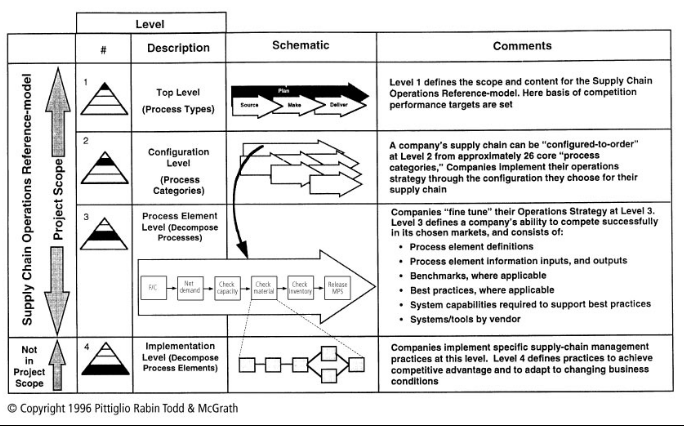
\includegraphics[width=.9\textwidth]{Stewart-1997.png}\\
  The four level model of SCOR as displayed in \cite{Stewart1997}
\end{center}

SCOR features four levels of supply-chain management:
\begin{itemize}
\item \textbf{Level 1} provides a broad definition of the plan, source, make,
  deliver process types, and is the point at which a company establishes its
  supply-chain competitive objectives.
\item \textbf{Level 2} defines 26 \emph{core process categories} that are
  possible components of a supply chain. A company can configure both its
  actual and ideal supply chain by selecting from these core processes.
\item \textbf{Level 3} provides a company with the information it needs to
  plan and set goals successfully for its supply-chain improvements through
  detailed process element information for each level 2 category. Planning
  elements include process element definitions, diagnostic metrics,
  benchmarks, best practices, and system software capabilities to enable best
  practices.
\item \textbf{Level 4} focuses on implementation, when companies put specific
  supply-chain improvements into play. Since changes at level 4 are unique to
  each company, the specific elements of the level are not defined within the
  industry-standard model.
\end{itemize}

SCOR focuses on four basic supply-chain processes:
\begin{itemize}
\item[(1)] \textbf{Plan:}
  \begin{itemize}
  \item \emph{Demand/supply planning:} Assess supply resources; aggregate and
    prioritize demand requirements; conduct inventory planning; assess
    distribution requirements; determine production, material, and rough-cut
    capacity for all products and all channels.
  \item \emph{Plan infrastructure:} Make/buy decisions; supply-chain
    configuration; long-term capacity and resource planning; business
    planning; product phase-in/phase-out; manufacturing ramp-up; end-of-life
    management; product line management.
  \end{itemize}
\item[(2)] \textbf{Source:}
  \begin{itemize}
  \item \emph{Sourcing/material acquisition:} Obtain, receive, inspect, hold
    and issue material.
  \item \emph{Source infrastructure:} Vendor certification and feedback;
    sourcing quality; inbound freight; component engineering; vendor
    contracts; initiation of vendor payment.  
  \end{itemize}
\item[(3)] \textbf{Make:}
  \begin{itemize}
  \item \emph{Production execution:} Request and receive material; manufacture
    and test product; package; hold and/or release product.
  \item \emph{Make infrastructure:} Engineering changes; facilities and
    equipment; production status; production quality; shop
    scheduling/sequencing; short-term capacity.
  \end{itemize}
\item[(4)] \textbf{Deliver:}
  \begin{itemize}
  \item \emph{Demand management:} Conduct forecasting; plan promotions; plan
    projects; plan sales campaigns; collect and analyse point of sale (POS)
    data and actual customer orders; promote products; price products; measure
    customer satisfaction; execute efficient customer response (ECR).
  \item \emph{Order management:} Enter and maintain orders; generate
    quotations; configure product; create and maintain customer database;
    manage allocations; maintain product/price database; manage accounts
    receivables, credits, collections and invoicing.
  \item \emph{Warehouse management:} Receive and stock finished goods; pick
    and pack; configure products; ship products; create customer specific
    package labelling; consolidate orders.
  \item \emph{Transportation management:} Manage traffic; manage freight;
    manage prod-uct import/export.
  \item \emph{Installation management:} Schedule installation activities;
    perform installation; verify performance.
  \item \emph{Deliver infrastructure:} Channel business rules; order rules;
    management of deliver inventories; management of deliver quantity.
  \end{itemize}
\end{itemize}

\begin{thebibliography}{xxx}
\bibitem{Bolstorff2017} Peter A. Bolstorff (2017).  20 Years of SCOR:
  Reflections on Relevancy and the Road Ahead. ASCM Blog, 03/27/2017.
  \url{https://www.ascm.org/}
  
\bibitem{Haertel2021} Stefan Härtel (2021). Slides to his talk on November 16,
  2021.  Available in the github repo.

\bibitem{Shchedrovitsky2004} Georgi P. Shchedrovitsky (2014). Selected Works.
  A Guide to the Methodology of Organisation, Leadership and Management. In:
  Khristenko, Reus, Zinchenko et al. Methodological School of Management.
  Bloomsbury Publishing.  ISBN 978-1-4729-1029-5.

\bibitem{Stewart1997} Gordon Stewart (1997). Supply-chain operations reference
  model (SCOR): the first cross-industry framework for integrated supply-chain
  management. Logistics Information Management, vol. 10 (2), pp. 62–67.
\end{thebibliography}

\end{document}

